\chapter{Fejlesztői dokumentáció} % Developer guide
\label{ch:developer}

\section{Keretrendszerek és az alkalmazás felépítése}
\label{sec:framework-app}
\subsection{Keretrendszerek}
\label{subsec:framework}
Az alkalmazás ASP.NET core 3.1 keretrendszerben készült \cite{ASPDOTNETCORE3_1}, ami egy nyílt forráskódú, webes alkalmazások készítésére szolgáló programkönyvtár, melyet a \emph{Microsoft} fejleszt. A keretrendszer lehetővé teszi, hogy az alkalmazás több platformon is tudjon futni (\emph{Linux}, \emph{macOS} és \emph{Windows}). Továbbá a \emph{Kendo UI Core for jQuery}\cite{KendoUIforJquery} keretrendszer biztosítja számunkra a felületen található felhasználóbarát táblázatokat, űrlap elemeket. A saját \emph{HTML} elemek stílusait a \emph{Bootstrap}\cite{Bootstrap} keretrendszer biztosítja.
\subsection{Az alkalmazás felépítése}
\label{subsec:app} 
Az alkalmazás az \emph{MVC} architektúrára épül (\ref{fig:mvc-pattern} ábra)\cite{MVC}. Tehát három rétegre bontható a felépítése, Modell-Nézet-Vezérlő. A Modell (angolul \emph{Model}) réteg tartalmazza az üzleti logikát, amely az adatokat kezeli és kapcsolatban van az adatbázissal. A nézet réteg (angolul \emph{View}) felelős a megjelenítésért. A vezérlő réteg (angolul \emph{Controller}) fogadja a kliens kéréseit és válaszol azokra. Az \emph{MVC} architektúra fő előnye, hogy jól elkülöníthetőek a rétegek, így a nézet független marad a modelltől. Ezáltal, ha szükséges, könnyedén le tudjuk cserélni az egész alkalmazás nézetét, vagy fordítva újra implementálhatjuk a modell réteg működését, anélkül hogy ez a nézeten bármi gondot okozna.
\begin{figure}[H]
	\centering
	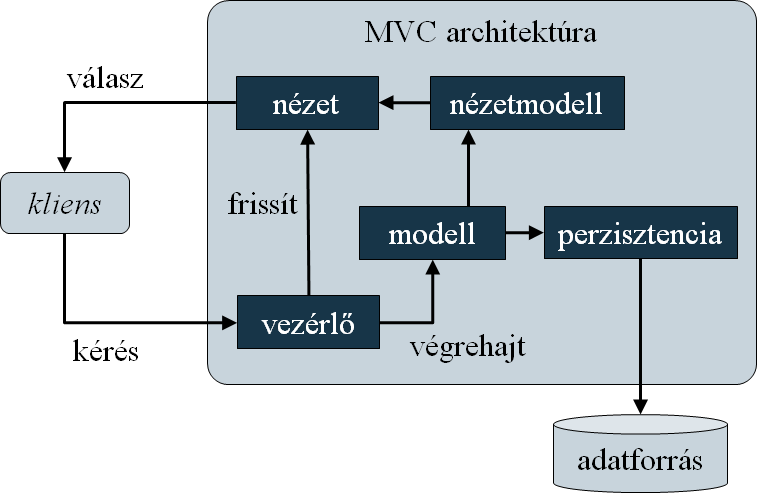
\includegraphics[width=1.0\textwidth]{developerguide/mvc-pattern}
	\caption{A Modell-Nézet-Vezérlő architektúra}
	\label{fig:mvc-pattern}
\end{figure}
Az alkalmazásban a könnyebb és egyszerűbb fejleszthetőség miatt a \emph{Model} réteget több komponensre bontjuk. Így az alábbi komponensekből áll össze a \emph{Model} réteg:
\begin{center}
	\begin{forest}
		for tree={
			font=\ttfamily,
			grow'=0,
			child anchor=west,
			parent anchor=south,
			anchor=west,
			calign=first,
			edge path={
			\noexpand\path [draw, \forestoption{edge}]
			(!u.south west) +(7.5pt,0) |- node[fill,inner sep=1.25pt] {} (.child anchor)\forestoption{edge label};
			},
			before typesetting nodes={
			if n=1
				{insert before={[,phantom]}}
				{}
			},
			fit=band,
			before computing xy={l=15pt},
		}
		[ASS
			[ASS.BLL/
				[Interfaces/]
				[Services/]
			]
			[ASS.DAL/
				[Models/]
				[ASSContext.cs]
				[DbInitializer.cs]
			]
			[ASS.WEB/
				[Models/
					[DTOs/]
					[ViewModels/]
				]
			]
		]
	\end{forest}
\end{center}
\begin{description}
	\item[ASS.BLL:]  az üzleti logikai réteget megvalósító komponens (angolul \emph{Business Logic Layer}).
	\item[ASS.DAL:] az adatelérési réteget megvalósító komponens (angolul \emph{Data Access Layer}).
	\item[ASS.WEB.Models:] ebben a komponensben tároljuk az adatok bevitelére és az adatok megjelenítésére szolgáló osztályokat.
	\item[ASSContext.cs:] az adatbázist leíró osztály.
	\item[DbInitializer.cs:] az adatbázist létrehozó statikus osztály.    
\end{description}
\section{Naplózás}
\label{sec:log}
Az alkalmazás fájl szintű naplózást tartalmaz, amit a \emph{Serilog.Extensions.Logging.File} nyílt forráskódú programkönyvtár használatával valósítjuk meg \cite{SERILOG}. Az alkalmazás automatikusan naplózza a futás közbeni eseményeket és az esetleges kivételeket. Természetesen támogatott a saját bejegyzések létrehozása is. A naplózás beállításait az \emph{appsettings.json} (\ref{src:json} ábra) fájlban tudjuk személyreszabni. Az alábbi négy értéket szabjuk személyre az alkalmazáshoz:
\begin{itemize}
	\item PathFormat: itt tudjuk megadni az alkalmazás naplófájljainak a mentési helyét, és egy sablont a fájlok nevére. A \emph{\{Date\}} paraméter helyére az aktuális dátum kerül beillesztésre (pl.: 20210513). Ha az elérési útban található mappa nem létezik azt a programkönyvtár automatikusan létrehozza a számunkra.
	\item OutputTemplate: itt adható meg a bejegyzések sablonja, hogy hogyan nézzenek ki a bejegyzés\footnote{\href{https://github.com/serilog/serilog/wiki/Formatting-Output}{Ezen a linken} részletes leírást olvashatunk az \emph{OutputTemplate}-ben használható paraméterekről.}. Az alkalmazás a következő sablont használja a bejegyzésekre: [\emph{Időbélyeg}] - [\emph{Esemény súlyossági szintje}] - [\emph{Üzenet}] \emph{Új sor} [\emph{Kivétel (ha van)}].
	\item LogLevel: itt állíthatjuk be, hogy milyen minimum szintű események kerüljenek naplózásra \cite{LogLevels}. A jelenlegi beállítással az alkalmazás minden legalább \emph{Information} szinttel rendelkező eseményt naplóz.
\end{itemize}
%\newpage
\lstset{caption={Naplózás beállításai}, label=src:log}
\begin{lstlisting}[language=json]
...
"Logging": {
	"PathFormat": "../Logs/log-{Date}.log",
	"OutputTemplate": "[{Timestamp:yyyy.MM.dd HH:mm:ss}] - [{Level:u}] - {Message}{NewLine}{Exception}",
	"LogLevel": {
		"Default": "Debug",
		"Microsoft": "Information"
	}
},
...
\end{lstlisting}
\section{Adatbázis}
\label{sec:database}
\subsection{Technológiák}
Az alkalmazáshoz szükséges telepítünk egy \emph{MySQL Community Server}-re, ajánlott a \emph{8.0.25}-ös verzió.\footnote{Az alkalmazás működik régebbi verzióval is. Viszont az alkalmazás nincs felkészítve az esetleges verziók közötti különbségekre.} Az autentikáció és autorizáció megvalósításához a Microsoft által készített \emph{Microsoft.AspNetCore.Identity.EntityFrameworkCore} nyílt forráskódú programkönyvtárat használja rendszer. A programkönyvtár tartalmaz meglévő adatbázis táblákat, melyeknek a tartalma és működése elolvasható a Microsoft hivatalos honlapján \cite{Identity}. A programkönyvtár gondoskodik a jelszavak biztonságos tárolásáról, melyet időfüggő sózással és a jelszó hashelésével valósít meg.

Az adatbázis \emph{code first} módszerrel van megvalósítva, tehát nem az adatbázis szerveren \emph{SQL} kódot futattva hozzuk létre az adatbázis táblákat, hanem modell osztályokkal definiáljuk az adatbázis táblákat \cite{CodeFirst}. Ezen modelleket az \emph{ASS.DAL.Models} névtérben tároljuk.

Az adatelérést az \emph{Entity Framework Core ORM} keretrendszer biztosítja \cite{EFCore}. Az objektum-relációs leképzés (angolul \emph{Object-Relational Mapping}), egy technika az adatok konvertálására nem kompatibilis típusos rendszerek és objektumorientált programozási nyelvek között. Így az alkalmazás forráskódjában nincsenek beégetett \emph{SQL} kódok. Ezek helyett a \emph{CRUD} (Create,Read,Update,Delete műveleteknek a rövidítése) műveleteket a \emph{.NET} nyújtotta és az \emph{Entity Framework Core} által is támogatott \emph{LINQ} (Language Integrated Queries) metódushívásokkal valósul meg \cite{LINQ}. Továbbá a keretrendszer védelmet biztosít az \emph{SQL Injection} támadások ellen \cite{SQLInjection}, ugyanis a műveletek a \emph{C\#} és \emph{LINQ} metódusokból kerülnek előállításra paraméterezetten.

Az adatbázis elérését az alkalmazás konfigurációs fájljában (\emph{appsettings.json}) tudjuk megadni illetve módosítani.
\lstset{caption={Adatbázis elérése}, label=src:dbconn}
\begin{lstlisting}[language=json]
...
"ConnectionStrings": {
	"DefaultConnection": "server=localhost;database=ASS;uid=username;password=fooBarraBoof"
},
...
\end{lstlisting}
\subsection{Adatbázis \emph{code first} objektumai}
A \emph{C\#} objektumok amelyekből az adatbázis képződik a \ref{fig:daldiagram} ábrán tekinthetjük meg. Maga az adatbázis az \emph{ASSContext} osztályból képződik. Minden egyes \emph{DbSet<T>}\footnote{Ahol a \emph{T} egy generikus típusparaméter.} típusú tulajdonság (angolul Property), egy adatbázis táblát jelent. Az osztály \emph{OnModelCreating} metódusában számos adatbázisra vonatkozó beállítást van lehetőségünk beállítani (pl.: táblák elsődleges kulcsai, külső kulcsai). A \emph{DbInitializer} osztály egy nyilvános \emph{Initialize} metódussal rendelkezik, mely létrehozza az adatbázis szerveren az adatbázist, ha még nem létezik, illetve a szükséges konstans adatokkal tölti fel az adatbázist (szerepkörök felvétele és rendszergazdai felhasználó létrehozása).
\begin{figure}[H]
	\centering
	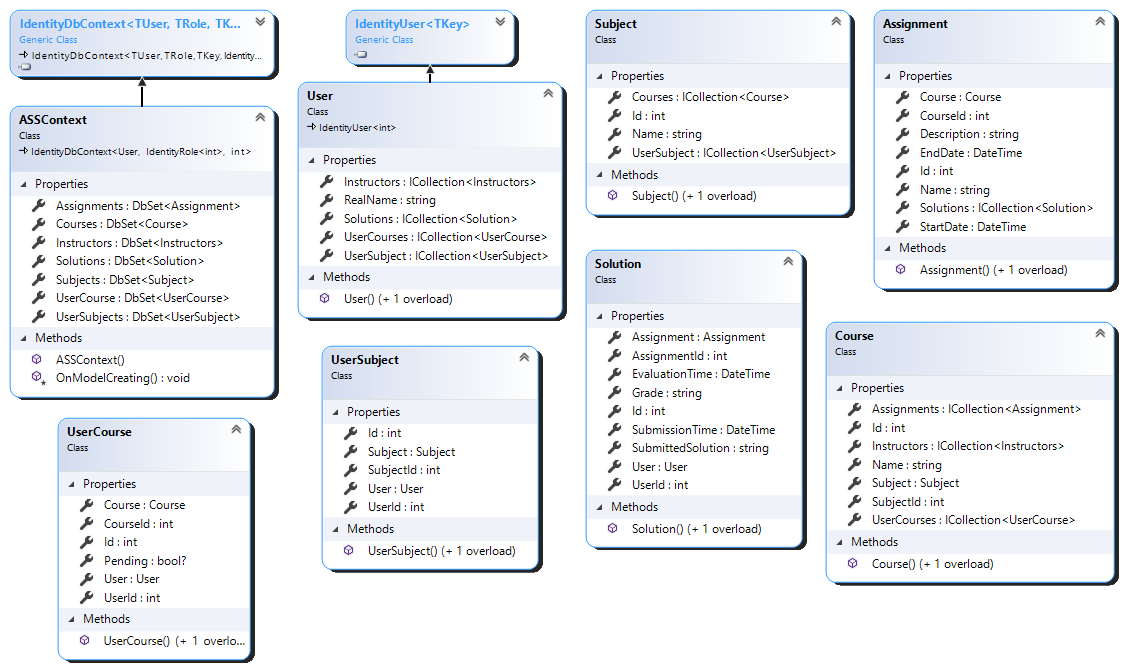
\includegraphics[width=1.0\textwidth]{developerguide/daldiagram}
	\caption{Az adatbázist leképző objektumok}
	\label{fig:daldiagram}
\end{figure}
\subsection{Az adatbázis táblái}
Az alkalmazás adatbázis diagramját a \ref{fig:dbdiagram} ábrán tekinthetjük meg. A \emph{Microsoft.AspNetCore.Identity.EntityFrameworkCore} keretrendszer által létrehozott táblákból csak azon a táblák és mezők kerülnek részletezésre, melyeket a rendszer aktívan használ. A táblák, amik nem kerülnek részletezésre a Microsoft hivatalos honlapján meg lehet tekinteni \cite{Identity}.
\begin{figure}[H]
	\centering
	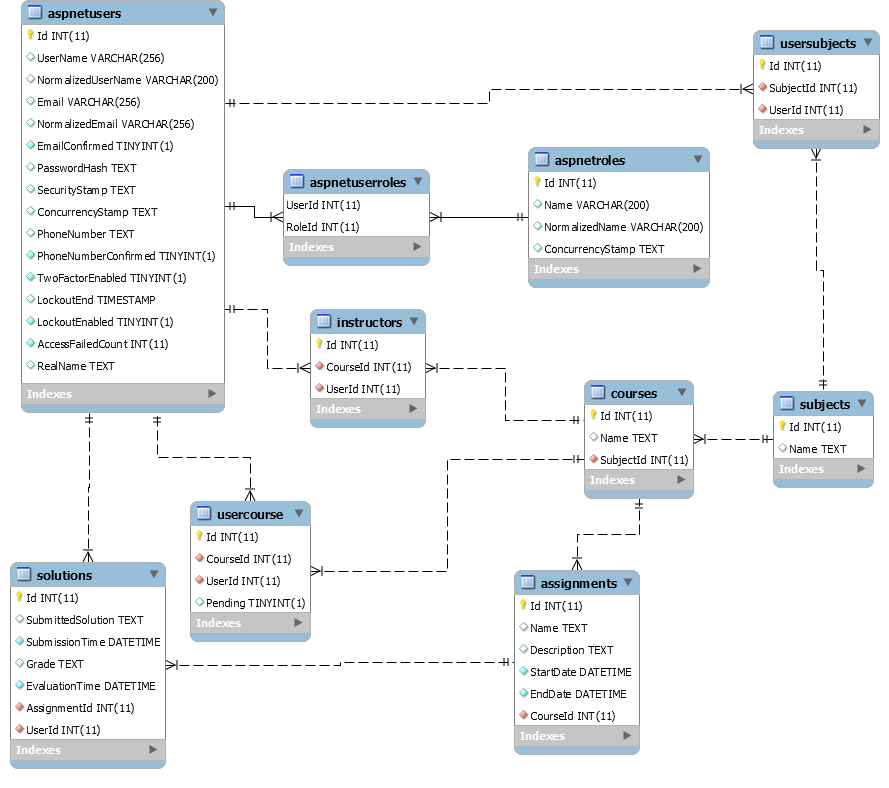
\includegraphics[width=1.0\textwidth]{developerguide/dbdiagram}
	\caption{Az adatbázis táblái}
	\label{fig:dbdiagram}
\end{figure}
\subsubsection{aspnetusers}
A \emph{Microsoft.AspNetCore.Identity.EntityFrameworkCore} programkönyvtár által automatikusan létrehozott tábla. A felhasználók adatait tárolja.
\begin{table}[H]
	\centering
	\begin{tabular}{ | m{0.25\textwidth} | m{0.25\textwidth} | m{0.40\textwidth} | }
		\hline
		\textbf{Mező neve} & \textbf{Típus} & \textbf{Leírás} \\
		\hline \hline
		Id & egész & Elsődleges kulcs \\
		\hline
		UserName & szöveg & Felhaszálónév (neptun kód) \\
		\hline
		Email & szöveg & Felhasználó e-mail címe \\
		\hline
		RealName & szöveg & Felhasználó neve \\
		\hline
		PasswordHash & szöveg & Felhasználó hashelt jelszava \\
		\hline
	\end{tabular}
	\caption{Adatbázis: felhasználók táblája}
	\label{tab:db-users}
\end{table}
\subsubsection{aspnetroles}
A \emph{Microsoft.AspNetCore.Identity.EntityFrameworkCore} programkönyvtár által automatikusan létrehozott tábla. A rendszerben használt szerepköröket tárolja.
\begin{table}[H]
	\centering
	\begin{tabular}{ | m{0.25\textwidth} | m{0.25\textwidth} | m{0.40\textwidth} | }
		\hline
		\textbf{Mező neve} & \textbf{Típus} & \textbf{Leírás} \\
		\hline \hline
		Id & egész & Elsődleges kulcs \\
		\hline
		Name & szöveg & Szerepkör megnevezése \\
		\hline
	\end{tabular}
	\caption{Adatbázis: szerepkörök táblája}
	\label{tab:db-roles}
\end{table}
\subsubsection{aspnetuserroles}
A \emph{Microsoft.AspNetCore.Identity.EntityFrameworkCore} programkönyvtár által automatikusan létrehozott tábla. Egy kapcsolótábla, mely tárolja a felhasználókhoz rendelt szerepköröket.
\begin{table}[H]
	\centering
	\begin{tabular}{ | m{0.25\textwidth} | m{0.25\textwidth} | m{0.40\textwidth} | }
		\hline
		\textbf{Mező neve} & \textbf{Típus} & \textbf{Leírás} \\
		\hline \hline
		UserId & egész & Elsődleges kulcs \\
		\hline
		RoleId & egész & Elsődleges kulcs \\
		\hline
	\end{tabular}
	\caption{Adatbázis: felhasználók és szerepkörök kapcsolótáblája}
	\label{tab:db-userroles-map}
\end{table}
\subsubsection{assignments}
Az \emph{assignments} tábla a csoportokhoz létrehozott beadandó feladatok adatainak tárolására szolgál.
\begin{table}[H]
	\centering
	\begin{tabular}{ | m{0.25\textwidth} | m{0.25\textwidth} | m{0.40\textwidth} | }
		\hline
		\textbf{Mező neve} & \textbf{Típus} & \textbf{Leírás} \\
		\hline \hline
		Id & egész & Elsődleges kulcs \\
		\hline
		Name & szöveg & A feladat neve \\
		\hline
		Description & szöveg & A feladat leírása \\
		\hline
		StartDate & dátum & A feladat elérésének dátuma \\
		\hline
		EndDate & dátum & A feladat határidejének dátuma \\
		\hline
		CourseId & egész & Arra vonatkozó kulcs, hogy a feladat melyik csoporthoz tartozik \\
		\hline
	\end{tabular}
	\caption{Adatbázis: feladatok táblája}
	\label{tab:db-assignments}
\end{table}
\subsubsection{courses}
A \emph{courses} tábla a tantárgyakhoz létrehozott csoportok adatait tárolja.
\begin{table}[H]
	\centering
	\begin{tabular}{ | m{0.25\textwidth} | m{0.25\textwidth} | m{0.40\textwidth} | }
		\hline
		\textbf{Mező neve} & \textbf{Típus} & \textbf{Leírás} \\
		\hline \hline
		Id & egész & Elsődleges kulcs \\
		\hline
		Name & szöveg & A csoport neve \\
		\hline
		SubjectId & egész & Arra vonatkozó kulcs, hogy a csoport melyik tantárgyhoz tartozik \\
		\hline
	\end{tabular}
	\caption{Adatbázis: csoportok táblája}
	\label{tab:db-courses}
\end{table}
\subsubsection{instructors}
A \emph{instructors} tábla egy kapcsolótábla, melyben a \emph{Gyakorlatvezető} szerepkörrel rendelkező felhasználókat kapcsoljuk a hozzájuk tartozó csoportokhoz. 
\begin{table}[H]
	\centering
	\begin{tabular}{ | m{0.25\textwidth} | m{0.25\textwidth} | m{0.40\textwidth} | }
		\hline
		\textbf{Mező neve} & \textbf{Típus} & \textbf{Leírás} \\
		\hline \hline
		Id & egész & Elsődleges kulcs \\
		\hline
		CourseId & egész & A csoportra vonatkozó kulcs \\
		\hline
		UserId & egész & A felhasználóra vonatkozó kulcs \\
		\hline
	\end{tabular}
	\caption{Adatbázis: gyakorlatvezetők táblája}
	\label{tab:db-instructors}
\end{table}
\subsubsection{solutions}
A \emph{solutions} tábla a feladatokra beadott megoldásokat tárolja.
\begin{table}[H]
	\centering
	\begin{tabular}{ | m{0.25\textwidth} | m{0.25\textwidth} | m{0.40\textwidth} | }
		\hline
		\textbf{Mező neve} & \textbf{Típus} & \textbf{Leírás} \\
		\hline \hline
		Id & egész & Elsődleges kulcs \\
		\hline
		SubmittedSolution & szöveg & A feladatra beadott megoldás \\
		\hline
		SubmissionTime & dátum & A megoldás beküldésének az időpontja \\
		\hline
		Grade & szöveg & A feladatra adott értékelése \\
		\hline
		EvaluationTime & dátum & A feladat értékelésének időpontja \\
		\hline
		AssignmentId & egész & Arra vonatkozó kulcs, hogy a megoldás melyik feladathoz tartozik\\
		\hline
		UserId & egész & Arra vonatkozó kulcs, hogy melyik felhasználó adta be a megoldást\\
		\hline
	\end{tabular}
	\caption{Adatbázis: megoldások táblája}
	\label{tab:db-solutions}
\end{table}
\subsubsection{subjects}
A \emph{subjects} tábla a rendszerben létrehozott tantárgyak adatait tárolja.
\begin{table}[H]
	\centering
	\begin{tabular}{ | m{0.25\textwidth} | m{0.25\textwidth} | m{0.40\textwidth} | }
		\hline
		\textbf{Mező neve} & \textbf{Típus} & \textbf{Leírás} \\
		\hline \hline
		Id & egész & Elsődleges kulcs \\
		\hline
		Name & szöveg & A tantárgy neve\\
		\hline
	\end{tabular}
	\caption{Adatbázis: megoldások táblája}
	\label{tab:db-subjects}
\end{table}
\subsubsection{usercourse}
A \emph{usercourse} tábla egy kapcsoló tábla, melyben a hallgatókat és a csoportok összerendelése valósul meg.
\begin{table}[H]
	\centering
	\begin{tabular}{ | m{0.25\textwidth} | m{0.25\textwidth} | m{0.40\textwidth} | }
		\hline
		\textbf{Mező neve} & \textbf{Típus} & \textbf{Leírás} \\
		\hline \hline
		Id & egész & Elsődleges kulcs \\
		\hline
		CourseId & egész & A csoportra vonatkozó kulcs\\
		\hline
		UserId & egész & A felhasználóra vonatkozó kulcs\\
		\hline
		Pending & igaz/hamis & Annak az értéke, hogy a felhasználónak a jelentkezése elfogadásra, vagy elutasításra került \\
		\hline
	\end{tabular}
	\caption{Adatbázis: hallgatók és csoportok kapcsolótáblája}
	\label{tab:db-usercourse}
\end{table}
\subsubsection{usersubjects}
A \emph{usersubjects} tábla egy kapcsoló tábla, melyben a tárgyfelelősök és a tantárgyak összerendelése valósul meg.
\begin{table}[H]
	\centering
	\begin{tabular}{ | m{0.25\textwidth} | m{0.25\textwidth} | m{0.40\textwidth} | }
		\hline
		\textbf{Mező neve} & \textbf{Típus} & \textbf{Leírás} \\
		\hline \hline
		Id & egész & Elsődleges kulcs \\
		\hline
		SubjectId & egész & A tantárgyra vonatkozó kulcs\\
		\hline
		UserId & egész & A felhasználóra vonatkozó kulcs\\
		\hline
	\end{tabular}
	\caption{Adatbázis: tárgyfelelősök és tantárgyak kapcsolótáblája}
	\label{tab:db-usersubjects}
\end{table}
\section{Model réteg}
\label{sec:model}
\subsection{Üzleti logika}
Az üzleti logikát megvalósító objektumokat az \emph{ASS.BLL.Interfaces} és az \emph{ASS.BLL.Services} névtérben tároljuk. Az üzleti logikát szerepkörökre bontva valósítjuk meg. Minden szerepkörhöz tartozik egy \emph{interface}, mely leírja a szerepkörhöz tartozó funkciók metódusait, valamint egy osztály, ami implementálja az adott \emph{interface}-t. Az \emph{interface}-ket megvalósító osztályok a \emph{BaseService} osztályból származnak le\footnote{Kivéve a \emph{LoginService} osztályt.} (\ref{fig:bll-baseservice} ábra), melyben azok a funkcionalitások kerültek implementálásra, amiket minden egyes szerepkörhöz tartozó \emph{service} osztálynak meg kell valósítania. Ezeket a \emph{service} osztályokat az alkalmazás \emph{IoC} (\emph{Inversion of Control}) konténerébe \cite{IoC} regisztráljuk. Ezáltal a vezérlő osztályok rendelkeznek a hozzájuk tartozó \emph{service} osztály egy példányával, melyet konstruktoron keresztüli függőségi befecskendezéssel kapnak meg. A vezérlő osztályok ezen \emph{service} osztályok metódusainak segítségével dolgozzák fel a kliens kéréseit és állítják elő a megfelelő válaszokat.
\begin{figure}[H]
	\centering
	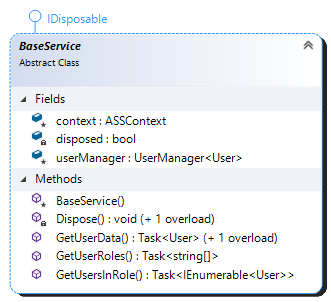
\includegraphics[width=0.7\textwidth]{developerguide/baseservice}
	\caption{Service osztályok őse}
	\label{fig:bll-baseservice}
\end{figure}
\subsubsection{BaseService osztály}
\begin{description}
	\item[GetUserData(ClaimsPrincipal):] paraméterül a bejelentkezett felhasználót\footnote{\href{https://docs.microsoft.com/en-us/dotnet/api/system.security.claims.claimsprincipal?view=netcore-3.1}{Ezen a linken} elolvashatjuk a \emph{ClaimsPrincipal} osztály dokumentációját.} kapja a metódus, majd eredményül a paraméterül kapott felhasználónak az adataival tér vissza.
	\item[GetUserData(int):] az előbbi metódus túlterhelése, itt a keresendő felhasználó egyedi kulcsát kapja a metódus paraméterül.
	\item[GetUserRoles(ClaimsPrincipal):] paraméterül a bejelentkezett felhasználót kapja, majd a felhasználó szerepköreivel tér vissza.
	\item[GetUsersInRole(Role):] paraméterül egy \emph{Role enum} értéket kap, majd a paraméterül kapott szerepkörrel rendelkező felhasználókkal tér vissza.
	\item[Dispose():] az \emph{IDisposeable interface} metódusa, mely gondoskodik a külső erőforrások felszabadításáról.
\end{description}
\subsubsection{LoginService osztály}
Ez az osztály felelős az alkalmazásba való bejelentkeztetésért, kijelentkeztetésért, valamint a bejelentkeztetett felhasználó fontos adatainak (felhasználónév, név, szerepkörök) lekérdezéséért, hogy a felhasználó munkamenetében (angolul \emph{session}) tudja tárolni a rendszer.
\begin{description}
	\item[CreateFullUserName(ClaimsPrincipal):] paraméterül a bejelentkezett felhasználót kapja, majd a felhasználó polgári nevéből és felhasználónevéből képzett \emph{string}-el tér vissza.
	\item[CreateUserRolesJson(ClaimsPrincipal):] paraméterül a bejelentkezett felhasználót kapja, majd a felhasználó szerepköreivel tér vissza.
	\item[SignIn(string,string,bool,bool):] paraméterül a bejelentkezési adatokat kapja, majd egy igaz/hamis értékkel tér vissza, ami a bejelentkezés sikerességét jelzi.
	\item[SignOut():] kijelentkezteti a felhasználót az alkalmazásból.
\end{description}
\begin{figure}[H]
	\centering
	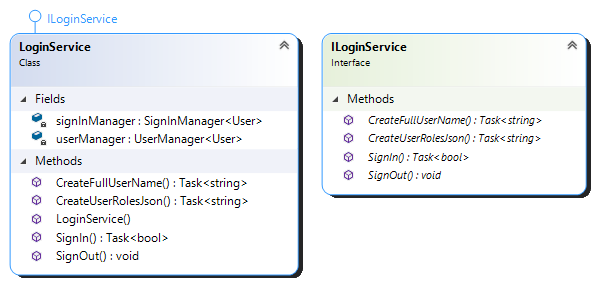
\includegraphics[width=1.0\textwidth]{developerguide/loginservice}
	\caption{LoginService osztály és interface}
	\label{fig:bll-loginservice}
\end{figure}
\subsubsection{AdminService osztály}
\begin{description}
	\item[CreateSubject(string{[]},string):] paraméterül \emph{tárgyfelelős}i szerepkörrel rendelkező felhasználók felhasználóneveit és a létrehozandó tantárgy nevét kapja. A metódus leellenőrzi, hogy a paraméterül kapott tantárgy név létezik-e már a rendszerben, ha nem, akkor a rendszer létrehozza a tantárgyat, egyébként kivétel váltódik ki.
	\item[GetSubjects():] a metódus visszatérési értéke a rendszerben létrehozott összes tantárgy.
	\item[UpdateSubject(int,string,string{[]}):] paraméterül egy tantárgy egyedi azonosítóját, tantárgy nevet és \emph{tárgyfelelős}i szerepkörrel rendelkező felhasználók felhasználóneveit kapja. A metódus módosítja a kapott paraméterek alapján a tantárgy adatait, ha az új tantárgynév még nem foglalt, egyébként kivétel váltódik ki.
	\item[DeleteSubject(int):] paraméterül egy tantárgy egyedi azonosítóját kapja, majd a megfelelő tantárgyat a metódus törli a rendszerből.
	\item[GetAllUser():] a metódus listázza a rendszerben tárolt összes felhasználót.
	\item[GetUserRoles(int):] paraméterül egy felhasználó egyedi azonosítóját kapja, majd a megfelelő felhasználó szerepköreivel tér vissza.
	\item[CreateUser(string,string,string,string,string{[]}):] a metódus egy új felhasználót hoz létre a rendszerben a paraméterül kapott adatok alapján.
	\item[UpdateUser(int,string,string,string,string{[]}):] paraméterül egy felhasználó adatait kapja (egyedi azonosító, felhasználónév, polgári név, e-mail cím, szerepkörök). A metódus a megfelelő felhasználó adatait módosítja.
\end{description}
\begin{figure}[H]
	\centering
	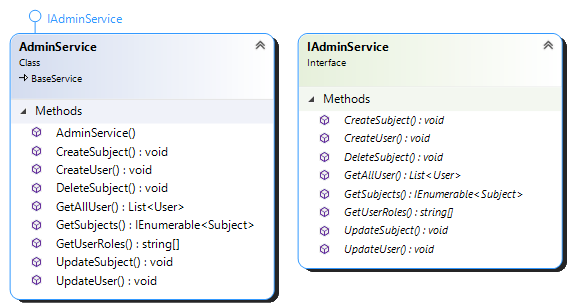
\includegraphics[width=1.0\textwidth]{developerguide/adminservice}
	\caption{AdminService osztály és interface}
	\label{fig:bll-adminservice}
\end{figure}
\subsubsection{TeacherService osztály}
Ez az osztály implementálja a \emph{tárgyfelelős}i szerepkörhöz tartozó funkciókat.
\begin{description}
	\item[CreateCourse(string{[]},int,string):] paraméterül felhasználónevek tömbjét, egy tantárgynak az egyedi azonosítóját illetve egy csoportnevet kap. A metódus létrehozza a paraméterül kapott tantárgyhoz az új csoportot, amennyiben ez lehetséges. Ha sikeres volt a csoport létrehozása, akkor a paraméterül kapott felhasználókat hozzárendeli a csoporthoz.
	\item[GetSubjects(ClaimsPrincipal):] paraméterül kap egy bejelentkezett felhasználót, majd a hozzárendelt tantárgyakkal tér vissza egy listában.
	\item[GetCourse(int):] paraméterül egy csoportnak az egyedi azonosítóját kapja, majd visszatér ezen csoport adataival.
	\item[EditCourse(int,string,string{[]}):] paraméterül egy csoportnak az egyedi azonosítóját, a csoport nevét, és gyakorlatvezetők felhasználóneveit kapja. A metódus a paraméterül kapott adatokkal módosítja a megfelelő csoportot. 
\end{description}
\begin{figure}[H]
	\centering
	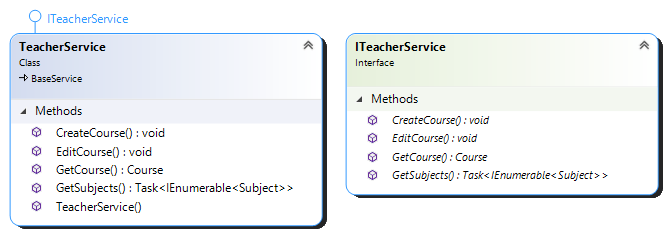
\includegraphics[width=1.0\textwidth]{developerguide/teacherservice}
	\caption{TeacherService osztály és interface}
	\label{fig:bll-teacherservice}
\end{figure}
\subsubsection{InstructorService osztály}
\begin{description}
	\item[GetPendingList(ClaimsPrincipal):] paraméterül a bejelentkezett felhasználót kapja, visszatérési értéke a felhasználóhoz tartozó csoportba jelenkezett hallgatók listája.
	\item[ProcessPendingStatus(int,bool):] paraméterül a jelentkezéseket tároló kapcsolótábla (\emph{UserCourses}) egyedi azonosítóját és egy igaz/hamis érték kap. A metódus az igaz/hamis érték alapján frissíti a megfelelő jelentkezési státuszt. Az igaz érték a jelentkezés elfogadását jelenti, a hamis pedig az elutasítást.
	\item[GetCourses(ClaimsPrincipal):] paraméterül a bejelentkezett felhasználót kapja, eredményül pedig a felhasználóhoz tartozó csoportokkal tér vissza.
	\item[CreateAssignment(string,string,DateTime,DateTime,int{[]}):] paraméterül egy feladatnak az adatait kapja. A metódus leellenőrzi, hogy a feladat elérésének a dátuma korábban van-e mint a beadási határidő, ha igen akkor elmenti a feladatot, ha nem teljesül a feltétel, akkor kivétel váltódik ki.
	\item[GetAssignment(int,int,ClaimsPrincipal):] paraméterül egy csoport és egy feladat egyedi azonosítóját valamint a bejelentkezett felhasználót kapja. A metódus a paraméterül kapott feladat adataival tér vissza, amennyiben a felhasználó gyakorlatvezetője a paraméterül kapott csoportnak, egyébként kivétel váltódik ki.
	\item[GetStudent(int):] paraméterül egy hallgató egyedi azonosítóját kapja, visszatérési értéke a megfelelő felhasználó adatai.
	\item[EvaluateAssignment(int,string,DateTime,ClaimsPrincipal):] paraméterül egy feladat egyedi azonosítóját, a feladatra beadott megoldás értékelését, az értékelésnek az időpontját és a bejelentkezett felhasználót kapja. A metódus ellenőrzi, hogy az a felhasználó, aki az értékelést végrehajtja, a kiiírt feladat csoportjának a gyakorlatvezetője-e. Ha igen, elmentődik az értékelés, egyébként kivétel váltódik ki.
\end{description}
\begin{figure}[H]
	\centering
	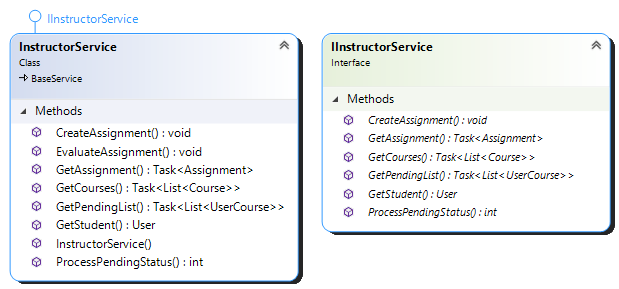
\includegraphics[width=1.0\textwidth]{developerguide/instructorservice}
	\caption{InstructorService osztály és interface}
	\label{fig:bll-instructorservice}
\end{figure}
\subsubsection{StudentService osztály}
Ez az osztály implementálja a \emph{hallgató}i szerepkörnek a funkcióit.
\begin{description}
	\item[GetCourses(ClaimsPrincipal):] paraméterül a bejelentkezett felhasználót kapja meg, majd a felhasználóhoz tartozó csoportokkal tér vissza.
	\item[CourseRegistration(int{[]},ClaimsPrincipal):] paraméterül csoportok egyedi azonosítójának a tömbjét és a bejelentkezett felhasználót kapja, majd a felhasználót felveszi a paraméterül kapott csoportokba\footnote{Ezen a ponton még a hallgató csak jelentkezést adott le az adott csoport(ok)ba.}.
	\item[Read\_AssignmentGrid(ClaimsPrincipal):] paraméterül a bejelentkezett felhasználót kapja, majd a hozzá tartozó csoportok listájával tér vissza.
	\item[GetAssignment(int,ClaimsPrincipal):] paraméterül egy feladatnak az egyedi azonosítóját és a bejelentkezett felhasználót kapja, majd visszatér a paraméterül kapott feladat adataival, ha a felhasználó tagja annak a csoportnak, amelyiket lekérdeztük.
	\item[SubmitSolution(int,ClaimsPrincipal,string,DateTime):] paraméterül egy feladat egyedi azonosítóját, a bejelentkezett felhasználót, a feladat megoldását és a beadás időpontját kapja. A metódus leellenőrzi, hogy a beadás időpontja korábbi-e mint a feladat beadási határideje. Amennyiben helyes a beadási idő, elmenti a beadott megoldást, ellenkező esetben kivétel váltódik ki.
\end{description}
\begin{figure}[H]
	\centering
	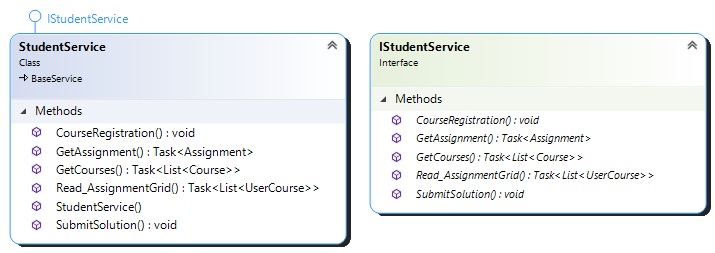
\includegraphics[width=1.0\textwidth]{developerguide/studentservice}
	\caption{StudentService osztály és interface}
	\label{fig:bll-studentservice}
\end{figure}
\subsection{Adatok megjelenítésére szolgáló modellek}
Az adatok megjelenítésére adatátviteli objektumok\footnote{\url{https://en.wikipedia.org/wiki/Data_transfer_object}} (angolul \emph{Data transfer object \(DTO\)}) kerülnek definiálásra. Feladatuk a folyamatok között közvetíteni a szükséges adatokat. Jelen esetben a vezérlő meghívja az üzleti logika megfelelő metódusát a kérés során, majd egy ilyen \emph{DTO} osztályba csomagolja az üzleti logika által visszaadott \emph{entitás}\todo{entitás objektum megdefiniálása} objektumokban tárolt adatokat és ezt az objektumot kapja meg a nézet, hogy megtudja jeleníteni a kliens számára az adatokat. Ezeket az osztályokat a \emph{ASS.WEB.Models.DTOs} névtérben tároljuk.
\subsection{Adatok bevitelére szolgáló modellek}
Az adatok bevitele nézetmodellek (angolul \emph{viewmodel}) segítségével valósul meg. A nézetmodelleket a \emph{ASS.WEB.Models.ViewModels} névtérben tároljuk. A nézetmodellek tulajdonságaira (angolul \emph{property}) megszabhatunk (egy vagy több) attribútomot, melyet a \emph{System.ComponentModel.DataAnnotations} névtérből érünk el. Az attribútomok használatával egyszerűen tudjuk validálni nézetmodelljeinket, vagy a valadiációs hibaüzenetek testreszabni. Ezt a \emph{.NET} keretrendszer biztosítja. Ugyanis fontos a felhasználó által kitöltött űrlapok ellenőrzése, hogy hibás adatok ne kerülhessenek a rendszerbe. A nézetmodelleket a rendszer az űrlapoknál használja fel, tehát a nézetmodellek egy-egy kitöltött űrlap adatait képes tárolni. Az attribútomok leírását a Microsoft hivatalos honlápján részletesen el lehet olvasni \cite{DataAnnotations}.
\lstset{caption={Példa az attribútomok használatára}, label=src:loginviewmodel}
\begin{lstlisting}[language={[Sharp]C}]
using System.ComponentModel.DataAnnotations;

namespace ASS.WEB.Models.ViewModels
{
	public class LoginViewModel
	{
		[Required(ErrorMessageResourceType = typeof(Resources.Models.ViewModels.LoginViewModel),ErrorMessageResourceName = "UsernameRequired")]
		[StringLength(maximumLength: 10, MinimumLength = 5, ErrorMessageResourceType = typeof(Resources.Models.ViewModels.LoginViewModel), ErrorMessageResourceName = "UsernameLengthMessage")]
		[Display(ResourceType = typeof(Resources.Models.ViewModels.LoginViewModel), Name = "Username")]
		public string Username { get; set; }

		[Required(ErrorMessageResourceType = typeof(Resources.Models.ViewModels.LoginViewModel), ErrorMessageResourceName = "PasswordRequired")]
		[StringLength(maximumLength: 30, ErrorMessageResourceType = typeof(Resources.Models.ViewModels.LoginViewModel),ErrorMessageResourceName = "PasswordLength")]
		[Display(ResourceType = typeof(Resources.Models.ViewModels.LoginViewModel), Name = "Password")]
		public string Password { get; set; }
	}
}
\end{lstlisting}
\subsection{Egyéb segédosztályok}
Az alkalmazásban definiálásra kerülnek egyéb segédosztályok és egy felsorolási típus (angolul \emph{enum}), melyeket az alább ábrán látható helyen találunk.
\begin{center}
	\begin{forest}
		for tree={
			font=\ttfamily,
			grow'=0,
			child anchor=west,
			parent anchor=south,
			anchor=west,
			calign=first,
			edge path={
			\noexpand\path [draw, \forestoption{edge}]
			(!u.south west) +(7.5pt,0) |- node[fill,inner sep=1.25pt] {} (.child anchor)\forestoption{edge label};
			},
			before typesetting nodes={
			if n=1
				{insert before={[,phantom]}}
				{}
			},
			fit=band,
			before computing xy={l=15pt},
		}
		[ASS
			[ASS.Common/
				[Enums/
					[Role.cs]
				]
				[Helpers/
					[CultureCodeMapping.cs]
				]
				[Settings/
					[IdentitySettings.cs]
					[LockoutSettings.cs]
					[PasswordSettings.cs]
					[UserSettings.cs]
				]
			]
		]
	\end{forest}
\end{center}
\subsubsection{Role.cs}
A \emph{Role} felsorolási típus segítségével definiáljuk a rendszerben tárolt szerepköröket. Ugyanis így a forráskódban nem szükséges beégetett szövegeket használnunk a szerepkörökre\footnote{Ez alól kivétel az \emph{Authorize} attribútom, mivel az attribútomokban a keretrendszer csak konstans értékeket enged használni.}.
\lstset{caption={Szerepkörök felsorolási típusa}, label=src:roleenum}
\begin{lstlisting}[language={[Sharp]C}]
namespace ASS.Common.Enums
{
	public enum Role
	{
		Admin,
		Teacher,
		Instructor,
		Student
	}
}
\end{lstlisting}
Továbbá a \emph{Role enum} segítségével egy ciklussal könnyedén tudjuk az adatbázisba perzisztálni az \emph{enum} értékeit.
\lstset{caption={Szerepkörök tárolása az adatbázisba (DbInitializer.cs)}, label=src:roles}
\begin{lstlisting}[language={[Sharp]C}]
...
foreach (Role item in Enum.GetValues(typeof(Role)))
{
	context.Roles.Add(new IdentityRole<int>() { Name = item.ToString(), NormalizedName = item.ToString() });
}
...
\end{lstlisting}
\subsubsection{CultureCodeMapping.cs}
A \emph{CultureCodeMapping} egy statikus segédosztály, amely egy nyelvi kódból a nyelvet adja vissza. Ezt a segédosztályt a lokalizációnál használjuk, hogy a felületen ne a nyelvi kód (pl.: \emph{hu-HU}) jelenjen meg, hanem az adott nyelv neve.
\lstset{caption={CultureCodeMapping osztály}, label=src:culturecodemapping}
\begin{lstlisting}[language={[Sharp]C}]
namespace ASS.Common.Helpers
{
	public static class CultureCodeMapping
	{
		public static string CultureCodeToCountryName(string cultureCode)
		{
			switch (cultureCode)
			{
				case "hu-HU":
					return "Magyar";
				case "en-US":
					return "English";
				default:
					return "Ismeretlen";
			}
		}
	}
}
\end{lstlisting}
\subsubsection{Settings osztályok}
A \emph{Microsoft.AspNetCore.Identity} \cite{IdentityOptions} lehetővé tesz különböző konfigurációk beállítását a felhasználói fiókokra. Például jelszóra vonatkozó konfigurációkat (minimum hossz, kötelező számot tartalmaznia stb), felhasználóra vonatkozó megszorításokat (minden felhasználó egyedi e-mail címmel rendelkezzen) és hibás bejelentkezés esetén konfigurálhatjuk a felhasználó kizárását az alkalmazásből (a kizárás időtartama). Ezen konfigurációk könnyű állíthatósága érdekében a konfigurációs értékek az alkalmazás konfigurációs fájljába (\emph{appsettings.json}) kiszervezésre kerültek.
\lstset{caption={Felhasználói fiók konfigurációs beállításai}, label=src:identityoptions}
\begin{lstlisting}[language=json]
...
"User": {
	"RequireUniqueEmail": false
},
"Password": {
	"RequiredLength": 1,
	"RequireLowercase": false,
	"RequireUppercase": false,
	"RequireDigit": false,
	"RequireNonAlphanumeric": false,
	"RequiredUniqueChars" : 1
},
"Lockout": {
	"AllowedForNewUsers": false,
	"DefaultLockoutTimeSpanInMins": 30,
	"MaxFailedAccessAttempts": 10
}
...
\end{lstlisting}
Ugyanis így a kód módosítása nélkül tudjuk változtatni ezen konfigurációs beállításokat és nem kell a változások után újra fordítani az alkalmazást, hanem elengedő csak újraindítani, hiszen a forráskód nem változott. Ezeket a beállításokat az alkalmazás indításakor kerül kiolvasásra az \emph{appsettings.json} fájlból, majd szerializálja a megfelelő objektumba (\emph{IdentitySettings} osztály) az adatokat. Továbbá egyszerre több fajta konfigurációs beállítást megadhatunk, annak függvényében, hogy az alkalmazás milyen módban fut\footnote{Ezt a beállítást is az \emph{appsettings.json} fájlban állíthatjuk} (\ref{src:appmode} forráskód).
\lstset{caption={Alkalmazás futási módja}, label=src:appmode}
\begin{lstlisting}[language=json]
"Mode": "Development",
...
\end{lstlisting}
Ennek használatával elég csak a módot változtatni, nem kell az összes \emph{IdentitySettings}-hez tartozó értéket módosítani.
\section{Vezérlő réteg}
\label{sec:controller}
\subsection{\emph{Home} vezérlő}
\subsection{\emph{Admin} vezérlő}
\subsection{\emph{Instructor} vezérlő}
\subsection{\emph{Teacher} vezérlő}
\subsection{\emph{Studnet} vezérlő}
\section{Nézet réteg}
\label{sec:view}
\subsection{\emph{Home} vezérlő nézetei}
\subsection{\emph{Admin} vezérlő nézetei}
\subsection{\emph{Instructor} vezérlő nézetei}
\subsection{\emph{Teacher} vezérlő nézetei}
\subsection{\emph{Student} vezérlő nézetei}
\subsection{Megosztott nézetek}
\section{Lokalizáció}
\label{sec:localization}